\section{Introduction}
\subsection{\textit{Data Mining}}
La création des systèmes de stockages, notamment des bases de données
a facilité la sauvegarde, l'organisation, et la recherche des données.
Ils ont évolués avec les objets que nous voulions stocker, qui sont de
plus en plus nombreux, complexes (types, structures, échelles, ...),
et par conséquent plus lourd. Le stockage massif de ces données est
motivé par de multiples raisons, par exemple, c'est simplement un
stockage d'éléments personnels (photos, vidéos, textes, ...), ou alors
des raisons professionnelles comme le suivi d'évolutions
(ventes de produit, ..) ou des changements (stockage de produits, ...)
ou d'autres encore.
Dans les raisons professionnelles, les données peuvent être utilisées
pour faire de la prise de décision. Cependant, dans ce cas précis,
deux problèmes surviennent. Premièrement les informations représentées
le sont sous formes de valeurs numériques, qui ne portent pas de
contexte, Il font donc l'extraire à partir des données brutes.
Deuxièmement avec l'augmentation croissante des données stockées,
l'analyse de patterns ou des contextes deviennent longue et complexe.
Les conclusions peuvent être fausses car induites en erreurs du à une
donnée inutile, ou elles peuvent être inexploitables dans la réalité.
Il faut réduire l'ensemble des données. La question suivante s'est
alors naturellement posée, comment comprendre ces données et les
transformer en informations c'est-à-dire en savoir exploitable et
utile. C'est dans ce contexte qu'est né le \textit{Data Mining}.
Le \textit{Data Mining} est "la pratique consistant à rechercher
automatiquement de grandes quantités de données afin de découvrir
des tendances et des modèles qui vont au delà de la simple analyse.
	[...]. Il est aussi connu sous le nom de découvert de connaissances
dans la données." \cite{oracle_data_mining}. Pour découvrir ce savoir,
il existe un processus, appelé \textit{Knowledge Discovery in Database} décrivant les étapes successives à faire (cf figure ci-dessous).

\begin{figure}[h!]
	\centering
	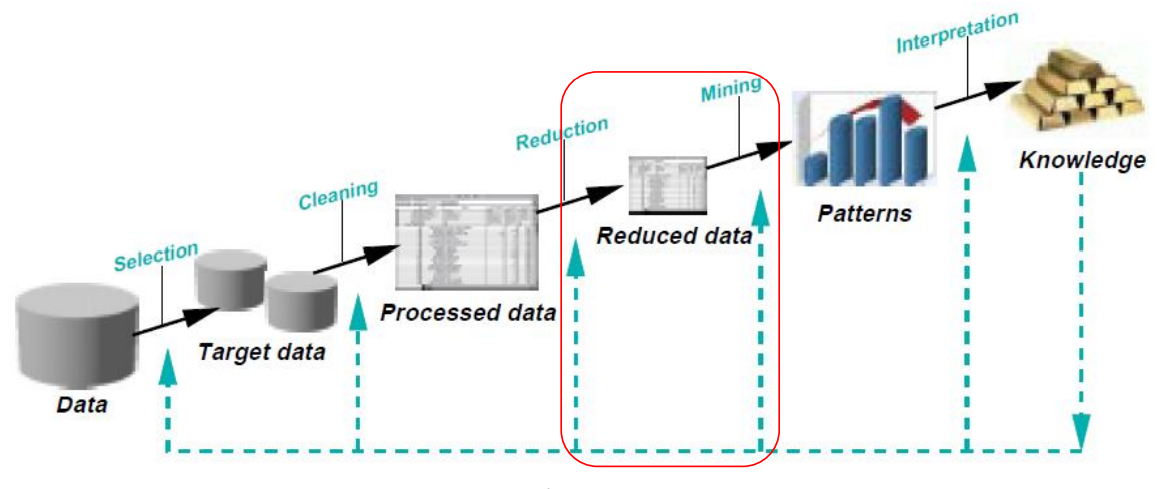
\includegraphics[scale=0.6]{img/kdd_process.png}
	\caption{KDD process}
	\label{fig:kdd_process}
\end{figure}

Dans ce papier nous nous concentrerons sur la partie \textit{Reduced Data}

\newpage
\subsection{\textit{Reduced Data}}
La réduction de dimentionalité (ou la selection de variable) est une
phasse très importantes du kDD. Elle a plusieurs objetifs, réduire le
nombre d'attributs afin d'accélérer l'apprentissage des modèles de
machine learning sur les données, selectionner les données les
plus importantes mais aussi apporter plus de sémantique aux données.
Pour faire de la réduction de donnée nous avons deux cas possibles,
soit nous souhaitons garder toutes les variables mais nous les
"simplifions" en les combinant. Cette méthode implique la perte de la
sémantique des données. Soit, à l'inverse, nous prenons uniquement les
variables les plus importantes et nous gardons la sémantique des
données.
La première s'appelle la \textit{transformation based}. Nous pouvons
citer comme exemple le \textit{Principal Component Analysis - PCA}.
Il va projeter les données sur des axes (les Composantes Principales)
en minimisant la distance entre les points et leurs projections.
Ainsi nous pouvons réduire notre problèmes de x variables à y
principales composantes. Nous devons aussi assurer que les données
garde une certaines sémantiques, nous ne voulons pas transformer nos
données n'importe comment. Dans le cas du \textit{PCA}, nous
calculons la variance cumulée et nous vérifions quelle soit entre
95\% et 99\%. Dans le cas de la prise de décision ne nous pouvons
pas appliquer une telle méthode car le sens des données nous importe.
La deuxième, la \textit{Selection based}, utilise des algorithmes
afin de connaître l'importance de chaque variable pour conserver
les plus importantes. Ici nous parlerons de l'une des méthodes
majeurs : le \textit{Rough Set theory - RST}.

\subsection{Contexte}
Ce travail est un projet réaliser par un étudiant en deuxième année
de master à l'université de Versailles Saint-Quentin en Yvelines.
Il est effectué dans le cadre d'une matière, "Projet conception et
programmation". Il est supervisé et sera évalué par ....
Les ojectifs de se travail sont multiples. Premièrement nous devons
comprendre comment fonctionne le \textit{QuickReduc}, un algorithme
basé sur le RST. Deuxièmement nous devons l'implémenter et le tester.
Troisièmement nous devons le comparer à d'autres algorithmes.
Pour cela nous commençerons par expliquer ce qu'est le RST. Ensuite
nous détaillerons sont fonctionnement, nous l'implémenterons et nous
le testerons sur des exemples simples. Puis nous appliquerons
plusieurs algorithmes similaires sur plusieurs \textit{datasets} et
nous les comparerons. Enfin nous conclurons. \\

\noindent
Commençons par expliquer ce qu'est le RST.